\documentclass[a4paper, 12pt]{article}%тип документа

%отступы
\usepackage[left=1.5cm,right=1cm,top=2cm,bottom=3cm,bindingoffset=0cm]{geometry}
\setlength{\parindent}{5ex}

%Русский язык
\usepackage[T2A]{fontenc} %кодировка
\usepackage[utf8]{inputenc} %кодировка исходного кода
\usepackage[english,russian]{babel} %локализация и переносы

%Вставка картинок
\usepackage{graphicx}
\graphicspath{{pictures/}}
\DeclareGraphicsExtensions{.pdf,.png,.jpg,.jfif}
\usepackage{wrapfig}

%Графики
\usepackage{pgfplots}
\pgfplotsset{compat=1.9}

%Математика
\usepackage{amsmath, amsfonts, amssymb, amsthm, mathtools}

%Таблицы
\usepackage{longtable} 
\usepackage{float}

%Римские цифры
\newcommand{\RomanNumeralCaps}[1]{\uppercase\expandafter{\romannumeral#1}}

\usepackage{multirow}


\begin{document}
	\begin{titlepage}
		\begin{center}
			\textsc{Федеральное государственное автономное образовательное учреждение высшего образования«Московский физико-технический институт (национальный исследовательский университет)»\\[5mm]
			}
			
			\vfill
			
			\textbf{Отчёт по лабораторной работе 5.10.1\\[3mm]
				Электронный парамагнитный резонанс
				\\[50mm]
			}
			
		\end{center}
		
		\hfill
		\begin{minipage}{.5\textwidth}
			Выполнили студенты:\\[2mm]
			Сериков Василий Романович\\[2mm]
			Сериков Алексей Романович\\[2mm]
			группа: Б03-102\\[5mm]
			
		\end{minipage}
		\vfill
		\begin{center}
			Москва, 2023 г.
		\end{center}
		
	\end{titlepage}
	
	\newpage
	\setcounter{page}{2}
	\textbf{Аннотация}\\
	
	\textbf{Цель работы: }\\
	
	 Исследование электронного парамагнитного резонанса (ЭПР) в молекуле ДФПГ, определить $g$-фактор электрона, измерить ширину линий ЭПР.\\
	
	\textbf{Теория: }\\
	
	В методе ЭПР изучается резонансное поглощение переменного электромагнитного поля в
	образце в зависимости от контролируемых экспериментатором внешних условий:
	постоянного магнитного поля, частоты колебаний переменного поля, температуры и так
	далее.
	
	Простейшей моделью для рассмотрения ЭПР является система из невзаимодействующих
	частиц со спином S=1/ 2 , помещённая во внешнее магнитное поле. В отсутствие
	магнитного поля энергии состояний с проекцией спина $S_z=\pm1/2$ совпадают. Из-за
	эффекта Зеемана энергии состояний с различными проекциями спина начинают различаться. Если направить на нашу систему поток излучения (поток фотонов) с энергией,
	равной разнице энергий этих состояний $h = g \mu_{B} B  $ , то станут возможны индуцированные
	переходы между состояниями. Эти переходы происходят с поглощением или
	испусканием фотона в зависимости от того, в каком из состояний была система до
	взаимодействия с излучением. В отличие от оптических переходов между электронными
	уровнями энергии в атоме, типичная частота переменного поля в ЭПР эксперименте
	составляет порядка 10 ГГц (а в нашем лабораторном эксперименте около 100 МГц), что
	соответствует энергии фотона менее 1К. Поэтому, за исключением очень низких температур,
	заселённость обоих спиновых подуровней с  $S_z=\pm1/2$ близка. В состоянии теплового
	равновесия нижний энергетический уровень более заселён, поэтому наблюдается
	поглощение электромагнитного излучения. 
	
	
	Поглощение переменного магнитного поля в образце описывается мнимой частью магнитной
	восприимчивости $P_{погл} = 0,5 \omega b^2\kappa^{''}(\omega\cdot B)$ , где $\omega$ — частота переменного поля, b —
	амплитуда однородного по малому образцу переменного поля и B — постоянное
	магнитное поле, а $\kappa^{''}$ — мнимая часть высокочастотной магнитной восприимчивости.
	В
	данной работе исследуется парамагнетик при комнатной температуре, восприимчивость и
	намагниченность которого в условиях эксперимента малы
	
	
	В «классическом» подходе рассматривается прецессия магнитного момента во внешнем поле при отклонении магнитного момента от равновесия. Классический магнитный диполь стремится выровняться вдоль силовых линий магнитного поля, при отклонении от равновесия возникает возвращающий механический момент $\mathbf{T} = \mathbf{M}\times \mathbf{B}$. Так как магнитный и механический момент иона связаны друг с другом гиромагнитным отношением $\gamma$ как $\mathbf{M}=\gamma \mathbf{J}$ , где $\mathbf{J}$ - это полный момент импульса, то с учётом уравнения динамики
	$\frac{d}{dt}\mathbf{J} = \mathbf{T}$, получим уравнение прецессии магнитного момента
	\[\dfrac{d}{dt}\mathbf{M} = \gamma \mathbf{M} \times \mathbf{B}.\] 
	Аналогично
	с известной задачей о прецессии гироскопа можно заметить, что при отклонении магнитного момента от направления магнитного поля возникает незатухающая прецессия вокруг направления поля с угловой скоростью $\boldsymbol{\Omega} = -\gamma \mathbf{B}$, частота этой прецессии $\Omega_L = \gamma B$ называется ларморовской. При совпадении частоты переменного поля, перпендикулярного основному, с ларморовской частотой возможно возникновение резонансного поглощения.\\
	
	\newpage
	
	\textbf{Описание установки: }\\
	
	\begin{figure}[H]
		\begin{center}
			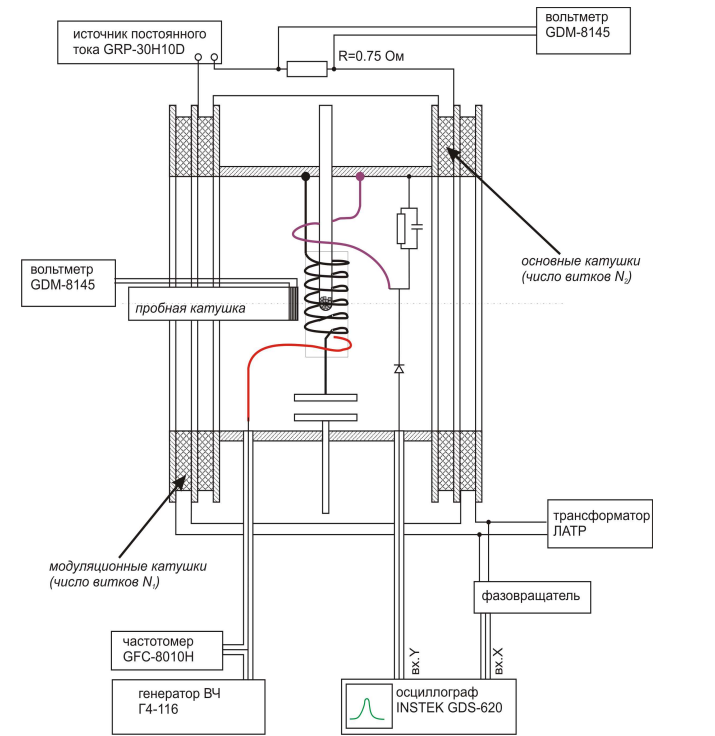
\includegraphics[width = 0.7\textwidth]{ust}
			\caption{Экспериментальная установка}
		\end{center}
	\end{figure}

	\begin{figure}[H]
		\begin{center}
			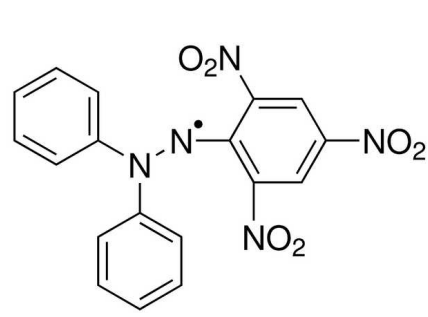
\includegraphics[width = 0.4\textwidth]{molecula}
			\caption{Химическая структура
				молекулы ДФПГ}
		\end{center}
	\end{figure}
	
	Схема установки представлена на Рис. 1. Образец (порошок ДФПГ) в стеклянной ампуле помещается внутрь катушки индуктивности, входящей в состав колебательного контура. Входящий в состав контура конденсатор состоит из двух пластин, разделённых воздушным зазором, одна из пластин может перемещаться поворотом штока. Колебания в контуре возбуждаются антенной, соединённой с генератором высокой частоты (ВЧ) Г4-116. Амплитуда колебаний поля в катушке индуктивности
	измеряется по наводимой в петле связи ЭДС индукции. Высокочастотные колебания ЭДС
	индукции в приёмном контуре детектируются диодом, измеряемая при помощи
	осциллографа низкочастотная огибающая этого сигнала пропорциональна квадрату
	амплитуды колебаний поля в катушке.\\
	
	Длина волны электромагнитного излучения на используемых в данной работе частотах ещё много больше размеров установки, поэтому можно считать, что потери в контуре определяются резистивными потерями в цепи и потерями на поглощение в исследуемом образце, а потери на излучение не учитывать.
	
	Средняя мощность резистивных потерь $P_R=\frac{1}{2} R_0 I^2$, где $R_0$ - сопротивление цепи контура, а $I$ - амплитудное значение тока в контуре.
	
	Мощность потерь в образце в условиях резонанса $P_{\text {поха }}=\frac{1}{2} \omega b^2 \chi^{\prime \prime}(\omega, B)$, для связи амплитуды колебаний поля $b$ с амплитудой тока в контуре $I$ воспользуемся тем, что в приближении длинной катушки $ \quad \Phi=n b S=\frac{1}{c} L I$ (СГС), где $L \quad$ - индуктивность катушки контура, а $n$ и $S$ - число витков в катушке и площадь её сечения.
	
	Таким образом, средняя поглощаемая мощность $\quad P_{\text {погл. }}=\frac{1}{2} \omega\left(\frac{L I}{c n S}\right)^2 \chi^{\prime \prime}(\omega, B)$. Поглощаемая мощность квадратична по току в катушке колебательного контура, как и резистивные потери в контуре. Поэтому для рассмотрения потерь и определения добротности контура с учётом поглощения мы можем рассматривать поглощение в образце как действие дополнительного сопротивления, «включаемого» в контур в момент наступления резонансного поглощения $\quad P_{\text {погл. }}=\frac{1}{2} R_{\text {ЭПР эфф } \phi} I^2$. Величина этого дополнительного сопротивления $R_{\text {ЭПР эфф }}=\omega\left(\frac{L}{c n S}\right)^2 \chi^{\prime \prime}(\omega, B)$
	
	Добротность последовательного колебательного контура $Q=\frac{1}{c R} \sqrt{\frac{L}{C}}=\frac{\omega_0 L}{c^2 R}$ (СГС), где $\omega_0=\frac{c}{\sqrt{L C}}\left(\right.$ СГС) - резонансная частота контура, а $R=R_0+R_{\text {ЭПР эфф }} \quad$ - полное сопротивление контура. В условиях опыта частота $\omega_0$ совпадает с частотой колебаний переменного поля $\omega$ и с ларморовской частотой $\Omega_L$.
	
	Амплитуда вынужденных колебаний при постоянной амплитуде раскачивающей силы пропорциональна добротности. Снимаемый детектором сигнал пропорционален квадрату амплитуды - то есть квадрату добротности. Тогда изменение сигнала при возникновении небольшого резонансного поглощения может быть связано с эффективным сопротивлением:
	
	и напряжение на детекторе в отсутствие поглощения в образце.
	Таким образом, относительное изменение сигнала на детекторе оказывается пропорционально мнимой части высокочастотной восприимчивости:
	$$
	\frac{\Delta U}{U_0}=2 Q_0 \frac{L}{(n S)^2} \chi^{\prime \prime} \quad \text { (СГC) }
	$$
	
	В системе СГС восприимчивость единицы объёма образца безразмерна, в эту формулу входит восприимчивость всего образца, её размерность $[\chi]=\mathrm{cm}^3$.
	
	Индуктивность катушки колебательного контура неизвестна, её можно оценить в приближении длинной катушки: $L=4 \pi n^2 S / l$ (СГС), где $l$ - длина катушки. С точностью этой оценки $\frac{\Delta U}{U} \simeq \frac{8 \pi Q_0}{S l} \chi^{\prime \prime}$.
	
	Таким образом, из амплитуды наблюдаемого сигнала ЭПР может быть определена абсолютная величина мнимой части восприимчивости в условиях резонансного поглощения.
	
	\newpage 
	
	\textbf{Ход работы: }\\
	
	\begin{enumerate}
		
		\item Определим резонансную частоту по наибольшей амплитуде огибающей модулированных колебаний генератора. $f_{\text{рез.}} = 124,32 \pm 0,01$ МГц.
		
		\item Измерим g-фактор электрона, для этого найдем значение индукции $B_0$ двумя способами. \\
		
		\textbf{i)} Расчет индукции постоянного поля по формуле для витка с током: 
		$$B= N\frac{\mu_0 I}{2r} $$
		
		где $\mu_0 = 4\pi \cdot 10^{-7}$ Ом$\cdot$с/м, $d_1$ = 0,28 мм,  $d_2$ = 0,31 мм -- диаметры витков, $N_1$ = 6700, $N_2$ = 5000\\
		Силу тока определим по закону Ома, зная сопротивление резистора $R = 0,75$ Ом. Значение напряжения на резисторе $U = 120$ мВ.
		
		Тогда рассчитаем величину магнитного поля:
		$$ B_1 = N_1\frac{\mu_0 I}{2r_1} = 5,4 \text{ Гс}$$
		$$ B_2 = N_2\frac{\mu_0 I}{2r_2} = 3,4 \text{ Гс}$$
				
		\textbf{ii)} Измерение переменного поля с помощью пробной катушки. Введем катушку внутрь основных катушек, измерим показания $U$ вольтметра, с которым соединена катушка. Зная число витков $N$ = 45, и площадь сечения $S = \pi d^2/4 = \pi 14,5^2 / 4 $ = (165 $\pm$ 2) мм$^2$ ($\sigma_d = 0,1$ мм), определим величину магнитного поля $B_0$ из соотношения:
		$$ U = NB_0S\omega_{\text{сеть}} $$
		
		где $\omega_{\text{сеть}}$ - угловая частота сети переменного тока.
		Значения напряжения получим с вольтметра при помещении катушки к основным катушкам.
		\begin{longtable}{|c|c|c|c|c|c|c|}
			\hline
			& \multicolumn{6}{c|}{u, мВ} \\ \hline
			у 1 осн. катушки & 1,40 & 1,41 & 1,40 & 1,41 & 1,41 & 1,41 \\ \hline
			у 2 осн. катушки & 1,49 & 1,49 & 1,49 & 1,49 & 1,49 & 1,49 \\ \hline
			\caption{Значения напряжений на пробной катушке при помещении ее к 1 и 2 основным катушкам. $\sigma_u = 0,01$ мВ}
		\end{longtable}
		Тогда из полученной таблицы получим среднее значение напряжения
		$$\overline{u} = \frac{1}{12} \sum_{i = 1}^{12} n_i = 1,45 \text{ мВ}$$
		
		$$ \sigma_{\overline{u}} = \sqrt{\frac{1}{12(12-1)} \sum_{i = 1}^{12} (\overline{x} - x_i)^2} = 0,01 \text{ мВ}$$
		
		$$ \sigma_{U} = \sqrt{\sigma_{\overline{u}}^2 + \sigma_{u}^2 } = 0,01 \text{ мВ}$$
		
		$$ U = 1,45 \pm 0,01 \text{ мВ} $$
		
		Тогда рассчитаем величину магнитного поля:
		$$ B_0 = 6,28 \text{ Гс}$$
		$$ \varepsilon_{B_0} = \sqrt{\varepsilon_U^2 + \varepsilon_S^2} = 1 \cdot 10^{-2} $$
		$$ \sigma_{B_0} = 0,06 \text{ Гс}$$
		
		
		\item Вычислим g-фактор для электрона с помощью формулы:
		
		$$ g = \frac{\hbar \omega_0}{\mu_{\text{Б}} {B_0}} = 2,27, \qquad \omega_0 = f_{\text{рез}} \cdot 2\pi$$
		
		%$$\overline{B} = 0,5 (B^i + B_0^{ii}) = 6,25 \text{ Гс}$$
		%$$ \sigma_{\overline {B}} = \sigma_{B_0^i}+ \sigma_{B_0^{ii}} = 0,08 \text{ Гс}$$
		$$ \sigma_g = g\sqrt{\varepsilon_{\omega_0}^2 + \varepsilon_{{B}}^2} = 0,03$$
		\item Определим ширину линии $\Delta B$ по формуле:
		
		$$ \Delta B /(2 B_{\text{мод.}}) = \Delta l / (2L) $$
		
		где $\Delta l$ - ширина линии поглощения на полувысоте кривой поглощения, \\
		а 2$L$ - полный размах по горизонтали луча осциллографа. \\
		
		
		$ B_{0} $ находится аналогично пункту 2. ii).
		\begin{longtable}{|c|c|c|c|c|c|c|}
			\hline
			& \multicolumn{6}{c|}{v, мВ} \\ \hline
			1 осн. катушка & 3,92 & 3,91 & 3,92 & 3,92 & 3,93 & 3,92 \\ \hline
			2 осн. катушка & 3,81 & 3,81 & 3,81 & 3,82 & 3,81 & 3,81 \\ \hline
			\caption{Значения напряжений на пробной катушке. $\sigma_v = 0,01$ мВ}
		\end{longtable}
		
		Аналогично пункту ii) рассчитаем среднее значение напряжения V:
			$$ B_{\text{0}}= 6,21 \text{ Гс} $$
		$$ \varepsilon_{B_{0}} = \varepsilon_V  = 1 \cdot 10^{-2} $$
		$$ \sigma_{B{0}} = 0,02 \text{ Гс}$$
		
		$$ V = 3,85 \pm 0,01 \text{ мВ} $$
		
		Тогда по полученным данным рассчитаем магнитное поле $B_{\text{мод.}}$:
	
		
		  Вольтметр измеряет действующее значение ЭДС индукции, а полный размах сигнала на экране осциллографа соответствует амплитудному значению переменного поля. По измеренной ЭДС индукции $V$ и параметрам катушки (числу витков $N$ = 45 и диаметру
		намотки d = 14,5 мм) определим амплитуду модулирующего поля 
		$$ B_{\text{мод}} = \sqrt{2} \cdot \frac{2V}{\pi^2 d^2 N \nu} = 2,33 \pm 0,01 \text{ Гс}$$ 
		где $\nu$ --
		частота модулирующего напряжения
		
		$$ \Delta B = 2 B_{\text{мод}}  \Delta l / (2L) = 0,87 \pm 0,08\text{ Гс}$$
		где $\Delta l $ = 1,5$\pm$0,2 дел. = 0,75$\pm$0,05 В, L = 4$\pm$0,2 дел. = 2,00 $\pm$0,05 В.
		
		Рассчитаем время релаксации из соотношения неопределенностей.
		$$ \Delta B g \mu_{\text{Б}} = E \approx h/\tau $$
		$$ \tau =  \frac{h}{\Delta B g \mu_{\text{Б}}} = 358 \pm 30\text{ нс} $$
		
			\begin{figure}[H]
			\begin{center}
				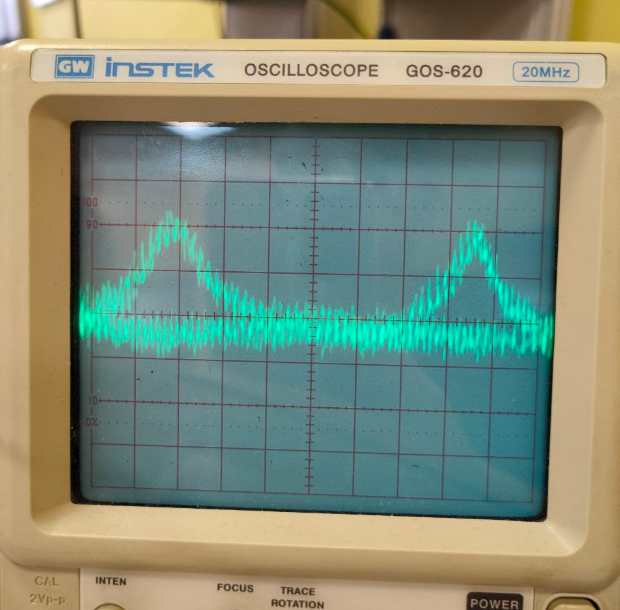
\includegraphics[width = 0.8\textwidth]{pict}
				\caption{Полученная осциллограмма для определения ширины ЭПР}
			\end{center}
		\end{figure}
		
		
		\textbf{Обсуждение результатов и выводы: }\\
		
		В ходе данной работы мы исследовали электронный парамагнитный резонанс в молекуле ДФПГ. Определили g-фактор электрона g = 2,27 $\pm$ 0,03. Теоретическое значение g = 2. Также измерили ширину линии ЭПР, полученное значение $\Delta B = 0,87 \pm 0,08$ Гс. Также определили время релаксации $\tau = 358 \pm 30 \text{ нс}$ 
		
		
		
		
		
		
		
		
		
		
		
		
		
		
		
		
		
		
		
		
		
		
		
		
		
		
		
		
		
		
		
		
	\end{enumerate}
	
	
	
	
	
	
	
	\end{document}